%====================================================
%
% Author: PR. XAVIER NOUMBISSI NOUNDOU
%
%====================================================
\documentclass[12pt, a4paper]{article}
\NeedsTeXFormat{LaTeX2e}

%---------------------------- PACKAGE INCLUSION -------------------------------
% This group renders characters clearer and more precise

\RequirePackage[bitstream-charter,cal,expert]{mathdesign}
\RequirePackage{latexsym}

\usepackage{geometry}
\geometry{a4paper,
		  %showframe=true,
		  %margin=2.75em,
		  %a4paper,
		  %total={170mm,257mm},
		  top=3.5em,
		  left=3em,
		  right=3em,
		  bottom=3.39em
		  }

\usepackage[default]{cantarell}
\usepackage{graphicx}
\usepackage{xspace}
\usepackage[parfill]{parskip} % Activate to begin paragraphs with an empty line rather than an indent
\usepackage{paralist} % very flexible & customisable lists (eg. enumerate/itemize, etc.)
\usepackage{listings} % for lstset definitions
\usepackage{url}
\usepackage{subfig} % make it possible to include more than one captioned figure/table in a single float
\usepackage{epsfig}
\usepackage{booktabs}
%\usepackage{enumitem} %funny itemize icons
\usepackage{verbatim}
\usepackage{tcolorbox}

\usepackage{pagecolor}

\usepackage{amsmath}
\newcommand{\mathbold}[1]{\text{\textbf{#1}}}

\usepackage{xcolor}
\definecolor{yerothColorOrange}{RGB}{242, 161, 0}   
\definecolor{yerothColorBlue}{RGB}{77 , 93 , 254}
\definecolor{yerothColorRed}{RGB}{254, 48 , 48}
\definecolor{yerothColorGray}{RGB}{198, 198, 198}
\definecolor{yerothColorDarkgray}{RGB}{60, 60 , 60}
\definecolor{yerothColorIndigo}{RGB}{83, 0, 125}
\definecolor{yerothColorGreen}{RGB}{2  , 160, 70}
\definecolor{forestgreen}{RGB}{2,160,70}    
\definecolor{mediumblue}{RGB}{7,43,205}    
\definecolor{firebrickred}{RGB}{178,34,34}
\definecolor{listingray}{gray}{0.9}
\definecolor{lbcolor}{rgb}{0.9,0.9,0.9}
\definecolor{darkgreen}{rgb}{0,0.35,0}
\definecolor{medgreen}{rgb}{0,0.5,0}
\definecolor{lightgreen}{rgb}{0.5,0.7,0.5}
\definecolor{pmcolour}{rgb}{0.5,0.7,0.5}
\definecolor{medgrey}{rgb}{0.6,0.6,0.6}
\definecolor{purplish}{rgb}{0.4,0,0.6}
\definecolor{brightred}{rgb}{1,0.2,0.2}

\newcommand{\diplinfn}{DR.\xspace}

\newcommand{\logicielerp}{syst\`eme--logiciel ERP\xspace}

\newcommand{\yerothrd}{\textcolor{yerothColorGreen}
			{\textsc{\textcolor{yerothColorRed}{YEROTH}}$_{\text{r\&d}}$\xspace}}

\newcommand{\yerotherpblack}{YEROTH--ERP--$3.0$\xspace}

\newcommand{\yerotherp}{\textcolor{yerothColorBlue}{\sc YEROTH--ERP--$3.0$}\xspace}

\newcommand{\saperp}{SAP Business One\xspace}

\newcommand{\sageerp}{Sage Gescom i$7$\xspace}

\newcommand{\myfullacademicname}{PR. XAVIER NOUMBISSI NOUNDOU\xspace}

\usepackage{hyperref}
\hypersetup{
    colorlinks,
	pagebackref,
    citecolor=medgreen,
    linkcolor=purplish,
    breaklinks,
    pdftex,
    bookmarks,
    plainpages=false,
	pdftitle={\yerotherp, comparaisons de syst\`emes--logiciels ERP,
	 		   \'edit\'e, par: ''\myfullacademicname''},
    pdfauthor={PR. XAVIER NOUMBISSI NOUNDOU}
}

%--------------------------------------------------------------------------------

%---------------------------- COMMANDS DEFINITION -------------------------------
\newcommand{\diplinf}{\emph{DR.}\xspace}

\newcommand{\emphbf}[1]{\textbf{#1}\xspace}
\newcommand{\emphit}[1]{\emph{\textit{#1}}\xspace}
\newcommand{\mycheckmark}[1]{\textcolor{#1}{$\checkmark$}\xspace}
\newcommand{\mytimes}[1]{\textcolor{#1}{$\times$}\xspace}
\newcommand{\boldsc}[1]{\textbf{\textsc{#1}}\xspace}

\newcommand{\myenumitem}[1]{\emph{#1}\xspace}
\newcommand{\yerothalert}{\emph{yeroth-erp-3-0-system-daemon}\xspace}

\newcommand{\mysql}{MySQL\xspace}
\newcommand{\mysqlcolored}{\textcolor{yerothColorBlue}{My}\textcolor{yerothColorOrange}{SQL}\xspace}

\newcommand{\role}{r\^ole\xspace}
\newcommand{\roles}{r\^oles\xspace}

\newcommand{\manager}{<< Manager >>\xspace}
\newcommand{\magasinier}{<< Magasinier >>\xspace}
\newcommand{\caissier}{<< Caissier >>\xspace}
\newcommand{\administrateur}{<< Administrateur >>\xspace}
\newcommand{\vendeur}{<< Vendeur >>\xspace}
\newcommand{\gestionairedestocks}{<< GestionaireDesStocks >>\xspace}

\newcommand{\qt}{Qt$5$\xspace}

\newcommand{\yerothfield}[1]{\textbf{\emph{#1}}\xspace}
\newcommand{\procparagraph}[1]
	{\paragraph{ \mycheckmark{forestgreen} \emph{\textcolor{forestgreen}{#1}}}}


\newcommand{\yerothvert}[1]{\textcolor{yerothColorGreen}{#1}\xspace}
\newcommand{\yerothorange}[1]{\textcolor{yerothColorOrange}{#1}\xspace}
\newcommand{\yerothrouge}[1]{\textcolor{yerothColorRed}{#1}\xspace}

\newcommand{\yerothevident}{\yerothvert{\'evidente}\xspace}
\newcommand{\yerothcompliquee}{\yerothorange{compliqu\'ee}\xspace}
\newcommand{\yerothtrescompliquee}{\yerothrouge{tr\`es compliqu\'ee}\xspace}



\newcommand{\featuresummary}[2]{\textbf{\textcolor{#1}{\textsc{#2}}}}

%--------------------------------------------------------------------------------

\usepackage[T1]{fontenc}
\newcommand{\changefont}[3]{
\fontfamily{#1} \fontseries{#2} \fontshape{#3} \selectfont}
\changefont{cmss}{m}{n}

% Set font to avant-garde
%\renewcommand*\rmdefault{pag}

\usepackage[french]{babel}
\addto\captionsfrench{\def\tablename{Tableau}}

\usepackage{fancyhdr}
\pagestyle{fancy}
\renewcommand{\headrulewidth}{0pt}
\rhead{}
\lhead{}
\lfoot{{\small Auteur: \myfullacademicname}}
\rfoot{{\small version du --~\today~--}}
\cfoot{}

%Remove widows and orphants
\clubpenalty = 10000
\widowpenalty = 10000
\displaywidowpenalty = 10000


\renewcommand\labelenumi{\theenumi)}

\pagenumbering{gobble}

\begin{document}

{\bf \Large \yerothrd} {| \sc \scriptsize Comparaisons avec quelques logiciels ERP}			
\\ \line(1,0){540}

\vspace{1.15em}


\parbox{27em}{\Large Avantages de \yerotherpblack Comparativement
				\`a \sageerp, et \`a \saperp}

\vspace{1em}

\begin{table}[!htbp]
\begin{tabular}{ll}
\parbox{27em}{
\yerotherp est un \logicielerp (Enterprise Resource Planing)
facile d'utilisation \`a cause de ses
caract\'eristiques suivantes:

\begin{enumerate}[1.]
	\itemsep -0.1em
	\item vue du logiciel d\'ependante du \role de l'utilisateur
	\item formation compl\`ete en $5$ jours
	\item interface du logiciel tr\`es facile \`a utiliser
	\item pas de connection internet requise
	\item pas de formation commerciale requise
	\item pas de formation comptable requise
	\item pas de formation universitaire requise. \\
\end{enumerate}
}

&

\parbox{15em}{
\begin{center}
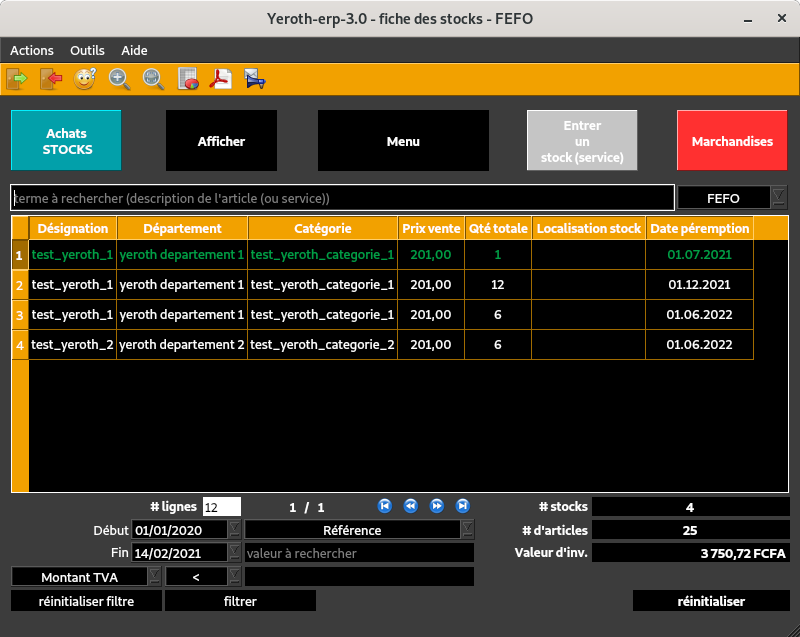
\includegraphics[scale=0.25]{images/yeroth-fenetre-stocks.png}
\caption*{La fiche des stocks}
\end{center}
}
\end{tabular}
\end{table}

\vspace{0cm}

Le tableau~\ref{tab:comparaisons-avec-quelques-logiciels-erp}
illustre \`a merveille la simplicit\'e et l'efficacit\'e
de \yerotherp, en comparaison avec les logiciels ERP ''\sageerp'',
et ''\saperp''.\\

\vspace{-1em}

\begin{table}[!htbp]
\selectlanguage{french}
\centering
\resizebox{\textwidth}{!}{%to fit the table within the text width
\begin{tabular}{cccc}

\multicolumn{1}{c}{}			&
\yerotherp 						& 
\sageerp						&
\saperp		\\ \hline

\textbf{vue du logiciel d\'ependante du \role}	&
		\yerothvert{OUI}				&
		\yerothvert{OUI}				&
		\yerothvert{OUI}				\\ \hline
		
\textbf{formation compl\`ete}		&
		\yerothvert{$5$ jours}			&
		\yerothorange{au moins $2$ mois}			&						
		\yerothrouge{au moins $3$ mois}			\\ \hline

\textbf{interface du logiciel}			&
		\yerothevident					&
		\yerothcompliquee				&						
		\yerothtrescompliquee				\\  \hline
		
\textbf{langage dans le logiciel}				&
		\yerothvert{usuel de tous les jours}	&
		\yerothorange{simple}					&						
		\yerothrouge{technique}					\\ \hline			
		
\textbf{formation comptable}	&
		\yerothvert{jamais}		&
		\yerothvert{jamais}		&						
		\yerothorange{utile}	\\ \hline		

\textbf{formation en marketing}	&
		\yerothvert{jamais}		&
		\yerothorange{utile}	&						
		\yerothorange{utile}	\\ \hline
		
\textbf{connection internet}		&
		\yerothvert{optionel}		&
		\yerothvert{optionel}		&						
		\yerothrouge{obligatoire}	\\		
\end{tabular}}
\caption{Comparaison entre \yerotherp et quelques autres logiciels ERP\\}
\label{tab:comparaisons-avec-quelques-logiciels-erp}
\end{table}

\vspace{1em}

{\large \bf OP\'ERATIONS}

\vspace{-0.05em}

\begin{table}[!htbp]
\begin{tabular}{lll}

\begin{tcolorbox}[width=14.3em, boxrule=0.01em, colback=white]
\textbf{Mat\'eriels~Point--de--Vente}
\vspace{0.1em}
\hrule
\vspace{0.25em}
\begin{itemize}[]
	\itemsep 0em
	\item[\mycheckmark{yerothColorDarkgray}] Lecteur de code--barres, etc.\\
\end{itemize}
\begin{center}
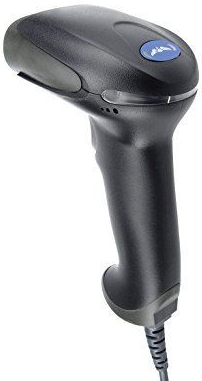
\includegraphics[scale=0.24]{images/xfox-fj-5-usb-plug-and-play-automatic-barcode-scanner.png}
\end{center}
\end{tcolorbox}

&

\begin{tcolorbox}[width=14.3em, boxrule=0.01em, colback=white]
\textbf{Syst\`emes--de--Gestion de Base--de--Donn\'ees}
\vspace{0.1em}
\hrule
\vspace{0.25em}
\begin{itemize}[]
	\itemsep 0em
	\item[\mycheckmark{yerothColorBlue}] \mysqlcolored\\
\end{itemize}
\begin{center}

\includegraphics[scale=0.164]{images/free-reuse-dbms-logo}
\end{center}
\end{tcolorbox}

&

\begin{tcolorbox}[width=14.3em, boxrule=0.01em, colback=white]
\textbf{Syst\`emes d'Exploitations}
\vspace{0.1em}
\hrule
\vspace{0.25em}
\begin{itemize}[]
	\itemsep 0em
	\item[\mycheckmark{yerothColorRed}] Debian--Linux\\
\end{itemize}
\begin{center}

\includegraphics[scale=0.53]{images/free-reuse-stretch-logo}
\end{center}
\end{tcolorbox}

\end{tabular}
\end{table}


\end{document}

